\documentclass[11pt,a4paper]{report}
\usepackage[textwidth=37em,vmargin=30mm]{geometry}
\usepackage{calc,xunicode,amsmath,amssymb,paralist,enumitem,tabu,booktabs,datetime2,xeCJK,xeCJKfntef,listings}
\usepackage{tocloft,fancyhdr,tcolorbox,xcolor,graphicx,eso-pic,xltxtra,xelatexemoji}

\newcommand{\envyear}[0]{2025}
\newcommand{\envdatestr}[0]{2025-04-22}
\newcommand{\envfinaldir}[0]{webdb/2025/20250422/final}

\usepackage[hidelinks]{hyperref}
\hypersetup{
    colorlinks=false,
    pdfpagemode=FullScreen,
    pdftitle={Web Digest - \envdatestr}
}

\setlength{\cftbeforechapskip}{10pt}
\renewcommand{\cftchapfont}{\rmfamily\bfseries\large\raggedright}
\setlength{\cftbeforesecskip}{2pt}
\renewcommand{\cftsecfont}{\sffamily\small\raggedright}

\setdefaultleftmargin{2em}{2em}{1em}{1em}{1em}{1em}

\usepackage{xeCJK,xeCJKfntef}
\xeCJKsetup{PunctStyle=plain,RubberPunctSkip=false,CJKglue=\strut\hskip 0pt plus 0.1em minus 0.05em,CJKecglue=\strut\hskip 0.22em plus 0.2em}
\XeTeXlinebreaklocale "zh"
\XeTeXlinebreakskip = 0pt


\setmainfont{Brygada 1918}
\setromanfont{Brygada 1918}
\setsansfont{IBM Plex Sans}
\setmonofont{JetBrains Mono NL}
\setCJKmainfont{Noto Serif CJK SC}
\setCJKromanfont{Noto Serif CJK SC}
\setCJKsansfont{Noto Sans CJK SC}
\setCJKmonofont{Noto Sans CJK SC}

\setlength{\parindent}{0pt}
\setlength{\parskip}{8pt}
\linespread{1.15}

\lstset{
	basicstyle=\ttfamily\footnotesize,
	numbersep=5pt,
	backgroundcolor=\color{black!5},
	showspaces=false,
	showstringspaces=false,
	showtabs=false,
	tabsize=2,
	captionpos=b,
	breaklines=true,
	breakatwhitespace=true,
	breakautoindent=true,
	linewidth=\textwidth
}






\newcommand{\coverpic}[2]{
    % argv: itemurl, authorname
    Cover photo by #2~~(\href{#1}{#1})
}
\newcommand{\makeheader}[0]{
    \begin{titlepage}
        % \newgeometry{hmargin=15mm,tmargin=21mm,bmargin=12mm}
        \begin{center}
            
            \rmfamily\scshape
            \fontspec{BaskervilleF}
            \fontspec{Old Standard}
            \fontsize{59pt}{70pt}\selectfont
            WEB\hfill DIGEST
            
            \vfill
            % \vskip 30pt
            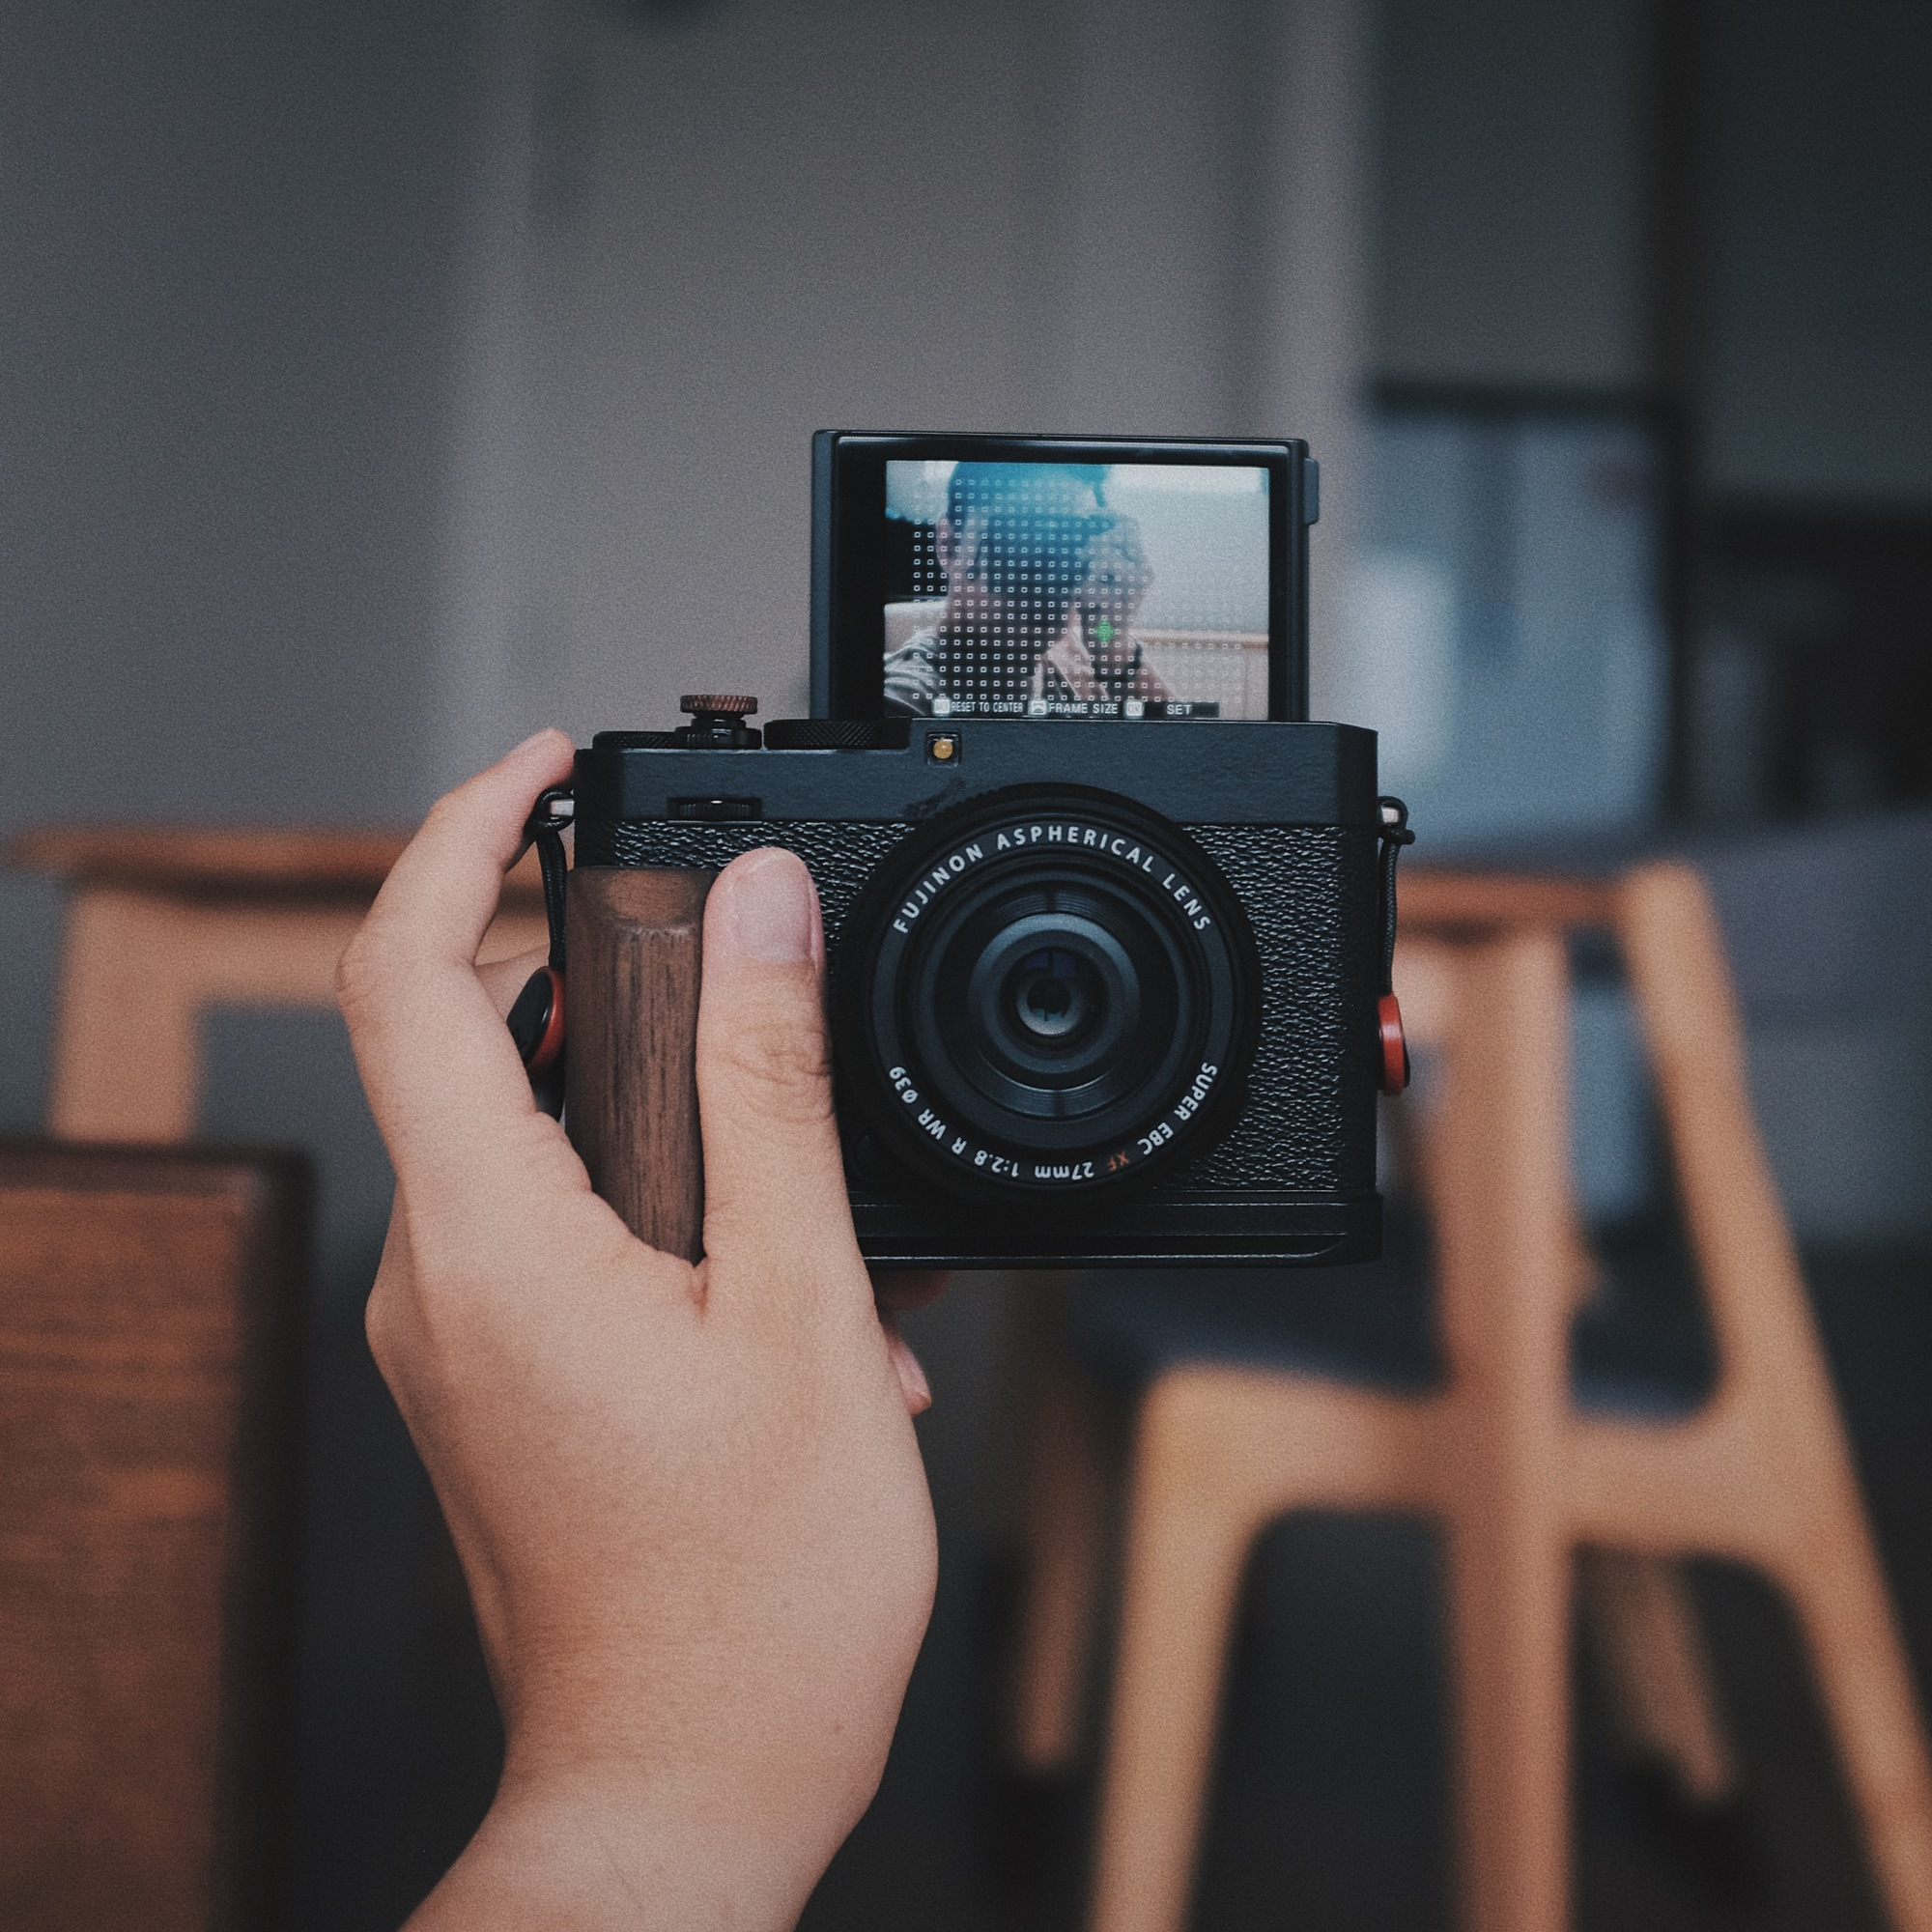
\includegraphics[width=\linewidth]{\envfinaldir/coverpic-prod.jpg}\par
            % \vskip 30pt
            \vfill

            \normalsize\rmfamily\scshape
            \copyright{} The Web Digest Project \hfill\large \envdatestr
        \end{center}
    \end{titlepage}
    % \restoregeometry
}
\newcommand{\simplehref}[1]{%
    \textcolor{blue!80!green}{\href{#1}{#1}}%
}
\renewcommand{\contentsname}{\center\Huge\sffamily\bfseries Contents\par\vskip 20pt}
\newcounter{ipartcounter}
\setcounter{ipartcounter}{0}
\newcommand{\ipart}[1]{
    % \vskip 20pt
    \clearpage
    \stepcounter{ipartcounter}
    \phantomsection
    \addcontentsline{toc}{chapter}{#1}
    % \begin{center}
    %     \Huge
    %     \sffamily\bfseries
    %     #1
    % \end{center}
    % \vskip 20pt plus 7pt
}
\newcounter{ichaptercounter}
\setcounter{ichaptercounter}{0}
\newcommand{\ichapter}[1]{
    % \vskip 20pt
    \clearpage
    \stepcounter{ichaptercounter}
    \phantomsection
    \addcontentsline{toc}{section}{\numberline{\arabic{ichaptercounter}}#1}
    \begin{center}
        \Huge
        \sffamily\bfseries
        #1
    \end{center}
    \vskip 20pt plus 7pt
}
\newcommand{\entrytitlefont}[1]{\subsection*{\raggedright\Large\sffamily\bfseries#1}}
\newcommand{\entryitemGeneric}[2]{
    % argv: title, url
    \parbox{\linewidth}{
        \entrytitlefont{#1}\par\vskip 5pt
        \footnotesize\ttfamily\mdseries
        \simplehref{#2}
    }\vskip 11pt plus 11pt minus 1pt
}
\newcommand{\entryitemGithub}[3]{
    % argv: title, url, desc
    \parbox{\linewidth}{
        \entrytitlefont{#1}\par\vskip 5pt
        \footnotesize\ttfamily\mdseries
        \simplehref{#2}\par\vskip 5pt
        \small\rmfamily\mdseries#3
    }\vskip 11pt plus 11pt minus 1pt
}
\newcommand{\entryitemAp}[3]{
    % argv: title, url, desc
    \parbox{\linewidth}{
        \entrytitlefont{#1}\par\vskip 5pt
        \footnotesize\ttfamily\mdseries
        \simplehref{#2}\par\vskip 5pt
        \small\rmfamily\mdseries#3
    }\vskip 11pt plus 11pt minus 1pt
}
\newcommand{\entryitemHackernews}[3]{
    % argv: title, hnurl, rawurl
    % \parbox{\linewidth}{
    %     \entrytitlefont{#1}\par\vskip 5pt
    %     \footnotesize\ttfamily\mdseries
    %     \simplehref{#3}\par
    %     \textcolor{black!50}{\href{#2}{#2}}
    % }\vskip 11pt plus 11pt minus 1pt
    \begin{minipage}{\linewidth}
            \entrytitlefont{#1}\par\vskip 5pt
            \footnotesize\ttfamily\mdseries
            \simplehref{#3}\par
            \textcolor{black!50}{\href{#2}{#2}}
    \end{minipage}\par\vskip 11pt plus 11pt minus 1pt
}







\begin{document}

\makeheader

\tableofcontents\clearpage




\ipart{Developers}
\ichapter{Hacker News}
\entryitemTwoLinks{Evertop: E-ink IBM XT clone with 100+ hours of battery life}{https://news.ycombinator.com/item?id=43757037}{https://github.com/ericjenott/Evertop}

\entryitemTwoLinks{Whistleblower statement on anomalies at time of DOGE work at NLRB [pdf]}{https://news.ycombinator.com/item?id=43755298}{https://whistlebloweraid.org/wp-content/uploads/2025/04/2025\_0414\_Berulis-Disclosure-HELP-and-Oversight-with-Exhibits.pdf}

\entryitemTwoLinks{Blog hosted on a Nintendo Wii}{https://news.ycombinator.com/item?id=43754953}{https://blog.infected.systems/posts/2025-04-21-this-blog-is-hosted-on-a-nintendo-wii/}

\entryitemTwoLinks{FTC takes action against Uber for deceptive billing and cancellation practices}{https://news.ycombinator.com/item?id=43754274}{https://www.ftc.gov/news-events/news/press-releases/2025/04/ftc-takes-action-against-uber-deceptive-billing-cancellation-practices}

\entryitemTwoLinks{Show HN: Dia, an open-weights TTS model for generating realistic dialogue}{https://news.ycombinator.com/item?id=43754124}{https://github.com/nari-labs/dia}

\entryitemTwoLinks{The campaign to subvert Africa's internet registry}{https://news.ycombinator.com/item?id=43753738}{https://www.capeindependent.com/article/the-campaign-to-subvert-africas-internet-registry}

\entryitemTwoLinks{A new form of verification on Bluesky}{https://news.ycombinator.com/item?id=43753651}{https://bsky.social/about/blog/04-21-2025-verification}

\entryitemTwoLinks{Out of the Fog}{https://news.ycombinator.com/item?id=43752532}{https://www.theverge.com/cs/features/651701/vietnam-operation-babylift-adoption-transnational}

\entryitemTwoLinks{LLM-powered tools amplify developer capabilities rather than replacing them}{https://news.ycombinator.com/item?id=43752492}{https://matthewsinclair.com/blog/0178-why-llm-powered-programming-is-more-mech-suit-than-artificial-human}

\entryitemTwoLinks{Handwriting activates broader brain networks than typing}{https://news.ycombinator.com/item?id=43752433}{https://www.psypost.org/handwriting-activates-broader-brain-networks-than-typing-study-shows/}

\entryitemTwoLinks{AI assisted search-based research works now}{https://news.ycombinator.com/item?id=43752262}{https://simonwillison.net/2025/Apr/21/ai-assisted-search/}

\entryitemTwoLinks{Launch HN: Magic Patterns (YC W23) – AI Design and Prototyping for Product Teams}{https://news.ycombinator.com/item?id=43752176}{https://news.ycombinator.com/item?id=43752176}

\entryitemTwoLinks{Pipelining might be my favorite programming language feature}{https://news.ycombinator.com/item?id=43751076}{https://herecomesthemoon.net/2025/04/pipelining/}

\entryitemTwoLinks{Fossil fuels fall below 50\% of US electricity for the first month on record}{https://news.ycombinator.com/item?id=43750617}{https://ember-energy.org/latest-updates/fossil-fuels-fall-below-50-of-us-electricity-for-the-first-month-on-record/}

\entryitemTwoLinks{Getting forked by Microsoft}{https://news.ycombinator.com/item?id=43750535}{https://philiplaine.com/posts/getting-forked-by-microsoft/}

\entryitemTwoLinks{Pope Francis has died}{https://news.ycombinator.com/item?id=43749449}{https://www.bbc.co.uk/news/live/crknlnzlrzdt}

\entryitemTwoLinks{Pope Francis has died}{https://news.ycombinator.com/item?id=43749405}{https://www.reuters.com/world/pope-francis-has-died-vatican-says-video-statement-2025-04-21/}

\entryitemTwoLinks{Reworking 30 lines of Linux code could cut power use by up to 30 percent}{https://news.ycombinator.com/item?id=43749271}{https://spectrum.ieee.org/data-center-energy-consumption}

\entryitemTwoLinks{Python's new t-strings}{https://news.ycombinator.com/item?id=43748512}{https://davepeck.org/2025/04/11/pythons-new-t-strings/}

\entryitemTwoLinks{The effect of deactivating Facebook and Instagram on users' emotional state}{https://news.ycombinator.com/item?id=43748486}{https://www.nber.org/papers/w33697}\ichapter{Phoronix}
\entryitemGeneric{\hskip 0pt{}Linux Patch Queued To Report Outdated Intel CPU Microcode As A Vulnerability}{https://www.phoronix.com/news/Intel-Old-Microcode-Vulnerable}

\entryitemGeneric{\hskip 0pt{}AMD ROCm 6.4 Adds SPIR-V Linking Support To HIP}{https://www.phoronix.com/news/AMD-ROCm-6.4-SPIR-V-Linker}

\entryitemGeneric{\hskip 0pt{}GCC Patch Revived For -mtune=generic Showing Nice Benefits On Intel \& AMD CPUs}{https://www.phoronix.com/news/GCC-Inline-Memset-Memcpy-Gen}

\entryitemGeneric{\hskip 0pt{}Ubuntu 25.04 vs. Windows 11 CPU Performance For The AMD Ryzen AI 7 PRO 360}{https://www.phoronix.com/review/ryzen-ai-7-pro-360-windows-linux}

\entryitemGeneric{\hskip 0pt{}Intel Posts Newest Code For Cache Aware Scheduling On Linux}{https://www.phoronix.com/news/Linux-RFC-Cache-Aware-Sched}

\entryitemGeneric{\hskip 0pt{}FamFS Ported To FUSE For Fabric-Attached Memory File-System}{https://www.phoronix.com/news/FamFS-FUSE-Patches}

\entryitemGeneric{\hskip 0pt{}RISC-V getrandom vDSO Ready Ahead Of Linux 6.16 With Exciting Performance}{https://www.phoronix.com/news/Linux-616-RISC-V-getrandom-vDSO}

\entryitemGeneric{\hskip 0pt{}Wine 10.6 Released With New Command Processor Lexer, 27 Bug Fixes}{https://www.phoronix.com/news/Wine-10.6-Released}

\entryitemGeneric{\hskip 0pt{}Linux 6.15-rc3 Released With GCC 15 Build Fixes, Intel Bartlett Lake \& Zen 5 Check}{https://www.phoronix.com/news/Linux-6.15-rc3-Released}\ichapter{Dribbble}
\entryitemGeneric{\hskip 0pt{}Tanuki - Raccoon, Animal Logo Design}{https://dribbble.com/shots/25917338-Tanuki-Raccoon-Animal-Logo-Design}

\entryitemGeneric{\hskip 0pt{}Cruising for the coast}{https://dribbble.com/shots/25914452-Cruising-for-the-coast}

\entryitemGeneric{\hskip 0pt{}Bismuth}{https://dribbble.com/shots/25918310-Bismuth}

\entryitemGeneric{\hskip 0pt{}Case study: Educational Website on Space Pollution}{https://dribbble.com/shots/25914349-Case-study-Educational-Website-on-Space-Pollution}

\entryitemGeneric{\hskip 0pt{}Columbus Rapids®}{https://dribbble.com/shots/25915181-Columbus-Rapids}

\entryitemGeneric{\hskip 0pt{}Cute Easter Bunny Mascot}{https://dribbble.com/shots/25914543-Cute-Easter-Bunny-Mascot}

\entryitemGeneric{\hskip 0pt{}UNIC // Mobile App}{https://dribbble.com/shots/25913185-UNIC-Mobile-App}

\entryitemGeneric{\hskip 0pt{}Phantom concept with Widget}{https://dribbble.com/shots/25911511-Phantom-concept-with-Widget}

\entryitemGeneric{\hskip 0pt{}Crypto Widget}{https://dribbble.com/shots/25913330-Crypto-Widget}

\entryitemGeneric{\hskip 0pt{}BB}{https://dribbble.com/shots/25913015-BB}

\entryitemGeneric{\hskip 0pt{}Startup Branding for Holidu: visual identity, brand design}{https://dribbble.com/shots/25903662-Startup-Branding-for-Holidu-visual-identity-brand-design}

\entryitemGeneric{\hskip 0pt{}Mountains to Sea}{https://dribbble.com/shots/25910072-Mountains-to-Sea}

\entryitemGeneric{\hskip 0pt{}Forg Logo}{https://dribbble.com/shots/25910287-Forg-Logo}

\entryitemGeneric{\hskip 0pt{}Cute Unicorn Mascot}{https://dribbble.com/shots/25909768-Cute-Unicorn-Mascot}

\entryitemGeneric{\hskip 0pt{}Logolounge Book 15 Entry - Client Work}{https://dribbble.com/shots/25909344-Logolounge-Book-15-Entry-Client-Work}

\entryitemGeneric{\hskip 0pt{}LéParc Logo Design - Boutique, Fashion Store, Letter L \& P Icon}{https://dribbble.com/shots/25908604-L-Parc-Logo-Design-Boutique-Fashion-Store-Letter-L-P-Icon}

\entryitemGeneric{\hskip 0pt{}Altitude}{https://dribbble.com/shots/25902364-Altitude}

\entryitemGeneric{\hskip 0pt{}Reindeer in Golden Light 🦌}{https://dribbble.com/shots/25905633-Reindeer-in-Golden-Light}

\entryitemGeneric{\hskip 0pt{}Automation builder - Wireframes}{https://dribbble.com/shots/25904187-Automation-builder-Wireframes}

\entryitemGeneric{\hskip 0pt{}Logo Collection > Birds Volume 03}{https://dribbble.com/shots/25905911-Logo-Collection-Birds-Volume-03}

\entryitemGeneric{\hskip 0pt{}Details - Amplemarket Logo \& Visual Identity}{https://dribbble.com/shots/25904732-Details-Amplemarket-Logo-Visual-Identity}

\entryitemGeneric{\hskip 0pt{}LogoLounge Book 15 Entry}{https://dribbble.com/shots/25904019-LogoLounge-Book-15-Entry}

\entryitemGeneric{\hskip 0pt{}FarmGirl Fresh®}{https://dribbble.com/shots/25905838-FarmGirl-Fresh}

\entryitemGeneric{\hskip 0pt{}Phantom components redesign≈}{https://dribbble.com/shots/25900820-Phantom-components-redesign}


\ipart{Developers~~~~(zh-Hans)}
\ichapter{Solidot}
\entryitemGeneric{\hskip 0pt{}群晖高端 NAS 产品只兼容其品牌硬盘}{https://www.solidot.org/story?sid=81104}

\entryitemGeneric{\hskip 0pt{}泰国政府利用人肉搜索压制异议}{https://www.solidot.org/story?sid=81103}

\entryitemGeneric{\hskip 0pt{}教宗方济各去世,享年 88 岁}{https://www.solidot.org/story?sid=81102}

\entryitemGeneric{\hskip 0pt{}旋转的宇宙或能解释哈勃张力}{https://www.solidot.org/story?sid=81101}

\entryitemGeneric{\hskip 0pt{}北极冬季海冰面积创卫星观测以来新低}{https://www.solidot.org/story?sid=81100}

\entryitemGeneric{\hskip 0pt{}亚马逊雨林的火融化了南极的冰}{https://www.solidot.org/story?sid=81099}

\entryitemGeneric{\hskip 0pt{}Blue95 Topanga 释出}{https://www.solidot.org/story?sid=81098}

\entryitemGeneric{\hskip 0pt{}马斯克的 DOGE 削减互联网档案馆的拨款}{https://www.solidot.org/story?sid=81097}

\entryitemGeneric{\hskip 0pt{}为避免撞上鹿芬兰给鹿角涂上反光漆}{https://www.solidot.org/story?sid=81096}

\entryitemGeneric{\hskip 0pt{}Arch Linux 成为最新一个用 Valkey 取代 Redis 的发行版}{https://www.solidot.org/story?sid=81095}

\entryitemGeneric{\hskip 0pt{}CA/Browser Forum 投票到 2029 年将证书有效期缩短至 47 天}{https://www.solidot.org/story?sid=81094}

\entryitemGeneric{\hskip 0pt{}研究发现五成员工使用未批准的 AI 工具}{https://www.solidot.org/story?sid=81093}

\entryitemGeneric{\hskip 0pt{}OpenAI 新推理模型有更高的幻觉比例}{https://www.solidot.org/story?sid=81092}

\entryitemGeneric{\hskip 0pt{}机器人在首届人机半程马拉松比赛中惨败给人类}{https://www.solidot.org/story?sid=81091}\ichapter{V2EX}
\entryitemGeneric{\hskip 0pt{}[问与答] 大家是怎么清理多年累积的照片的?}{https://www.v2ex.com/t/1127157}

\entryitemGeneric{\hskip 0pt{}[问与答] 除了 deepl,有没有其他翻译质量较好的免费服务}{https://www.v2ex.com/t/1127155}

\entryitemGeneric{\hskip 0pt{}[程序员] 请教一下存储大佬, 这服务器的硬盘是不是很快要升天了? 有必要立刻迁移数据吗?}{https://www.v2ex.com/t/1127153}

\entryitemGeneric{\hskip 0pt{}[推广] PICSPOT - 瞬息归档,恒久留存}{https://www.v2ex.com/t/1127152}

\entryitemGeneric{\hskip 0pt{}[Instagram] instagram 登入地区判定点解}{https://www.v2ex.com/t/1127151}

\entryitemGeneric{\hskip 0pt{}[分享创造] 我用 Rust 写了一个日漫汉化工具}{https://www.v2ex.com/t/1127149}

\entryitemGeneric{\hskip 0pt{}[问与答] 男方妈妈让还房贷,同意吗?}{https://www.v2ex.com/t/1127148}

\entryitemGeneric{\hskip 0pt{}[问与答] 如何用 AI 做翻译? 有没有大佬分享个 prompt 之类的}{https://www.v2ex.com/t/1127145}

\entryitemGeneric{\hskip 0pt{}[分享创造] [开源]Claude 历史对话下载器}{https://www.v2ex.com/t/1127143}

\entryitemGeneric{\hskip 0pt{}[问与答] 腾讯身份验证器小程序在通用中清除缓存后丢失所有令牌🤬}{https://www.v2ex.com/t/1127142}

\entryitemGeneric{\hskip 0pt{}[分享创造] 为腾讯云对象存储(COS)打造的高效图片管理工具}{https://www.v2ex.com/t/1127141}

\entryitemGeneric{\hskip 0pt{}[问与答] 请问一下,国内的 APP 上架应用商城这些,个体户与有限公司,这些区别大吗?}{https://www.v2ex.com/t/1127140}

\entryitemGeneric{\hskip 0pt{}[创业组队] [创业组队] 寻``不安分的心''}{https://www.v2ex.com/t/1127139}

\entryitemGeneric{\hskip 0pt{}[职场话题] 深圳 Java 今年工作好难找啊,一个 offer 没有}{https://www.v2ex.com/t/1127138}

\entryitemGeneric{\hskip 0pt{}[分享发现] Vue 3 轻量级闪卡学习应用(氛围编程开源应用)}{https://www.v2ex.com/t/1127136}

\entryitemGeneric{\hskip 0pt{}[问与答] h5 端美团外卖/饿了么可以查看到``我的评价''吗?}{https://www.v2ex.com/t/1127135}

\entryitemGeneric{\hskip 0pt{}[问与答] 深夜帮大龄程序员解决问题,有感而发。}{https://www.v2ex.com/t/1127134}

\entryitemGeneric{\hskip 0pt{}[问与答] 有没有腾讯安全反诈骗实验室的朋友}{https://www.v2ex.com/t/1127133}

\entryitemGeneric{\hskip 0pt{}[问与答] 公司主域名到底用什么呢?}{https://www.v2ex.com/t/1127132}

\entryitemGeneric{\hskip 0pt{}[生活] 我和对象谈好彩礼钱了,结果女方母亲和我爸打电话吵了一架}{https://www.v2ex.com/t/1127130}

\entryitemGeneric{\hskip 0pt{}[Nintendo Switch] NSO 普通家庭组会员 1 车位}{https://www.v2ex.com/t/1127129}

\entryitemGeneric{\hskip 0pt{}[程序员] 使用 VSCode 接入 DeepSeek V3 平替 Cursor 与 Trae 的 AI 编程方案}{https://www.v2ex.com/t/1127128}

\entryitemGeneric{\hskip 0pt{}[剧集] 推荐迷雾剧场新剧《借命而生》}{https://www.v2ex.com/t/1127127}

\entryitemGeneric{\hskip 0pt{}[问与答] 怎么开始 3D 打印?}{https://www.v2ex.com/t/1127126}

\entryitemGeneric{\hskip 0pt{}[程序员] [15-20K+期权] futter/rn 全栈开发工程师,远程全职}{https://www.v2ex.com/t/1127124}

\entryitemGeneric{\hskip 0pt{}[iPhone] 苹果的隔空投送做的越来越烂了}{https://www.v2ex.com/t/1127123}

\entryitemGeneric{\hskip 0pt{}[iPhone] 没人吐槽 iPhone 会自动删除通话记录吗}{https://www.v2ex.com/t/1127122}

\entryitemGeneric{\hskip 0pt{}[Apple] MacOS 的快捷键的逻辑在哪里?}{https://www.v2ex.com/t/1127121}

\entryitemGeneric{\hskip 0pt{}[Tesla] 单踏板模式北京早高峰通勤}{https://www.v2ex.com/t/1127120}

\entryitemGeneric{\hskip 0pt{}[算法] 跪求大佬指点! 10GB+数据查重最优解,哪种算法能扛住?}{https://www.v2ex.com/t/1127118}

\entryitemGeneric{\hskip 0pt{}[NAS] 家用全闪存 NAS 推荐}{https://www.v2ex.com/t/1127116}

\entryitemGeneric{\hskip 0pt{}[分享发现] 旅拍无人机推荐}{https://www.v2ex.com/t/1127115}

\entryitemGeneric{\hskip 0pt{}[问与答] WordPress 自定义字体,但是忘了字体文件在哪...}{https://www.v2ex.com/t/1127114}

\entryitemGeneric{\hskip 0pt{}[Java] 权限模型中的 基于角色的访问控制(RBAC)和基于属性的访问控制(ABAC)这两种怎么结合一起使用}{https://www.v2ex.com/t/1127113}

\entryitemGeneric{\hskip 0pt{}[问与答] 有没有谁了解民办中职/中专盈利情况的?}{https://www.v2ex.com/t/1127111}

\entryitemGeneric{\hskip 0pt{}[VXNA] 申请收录|雾语 - 迷雾轻语,雅意深藏}{https://www.v2ex.com/t/1127110}

\entryitemGeneric{\hskip 0pt{}[全球工单系统] cloud.dify.ai 挂了吗?}{https://www.v2ex.com/t/1127108}

\entryitemGeneric{\hskip 0pt{}[投资] 金价大涨,一直历史新高,还能上车吗?}{https://www.v2ex.com/t/1127107}

\entryitemGeneric{\hskip 0pt{}[职场话题] 三方协议签署前未告知违约金金额,签署后才知数额,是否具有法律效力?​}{https://www.v2ex.com/t/1127106}

\entryitemGeneric{\hskip 0pt{}[酷工作] web3 行业,远程, 4-6k/u 月薪 招 D3/threejs/WEBgl 动画前端开发}{https://www.v2ex.com/t/1127105}

\entryitemGeneric{\hskip 0pt{}[程序员] ArkFlow - 高性能 Rust 流处理引擎,在下一个版本中可扩展性将得到极大提升!}{https://www.v2ex.com/t/1127104}

\entryitemGeneric{\hskip 0pt{}[分享发现] 各位独立开发者还是需要稍稍警惕中间人攻击}{https://www.v2ex.com/t/1127103}

\entryitemGeneric{\hskip 0pt{}[Apple] 近万元的 Windows 轻薄本,除了它是 Windows,拿什么和 MBA 打?}{https://www.v2ex.com/t/1127102}

\entryitemGeneric{\hskip 0pt{}[问与答] cursor pro 年度会员市场价是多少?}{https://www.v2ex.com/t/1127101}

\entryitemGeneric{\hskip 0pt{}[Apple] craft 笔记应用五折了}{https://www.v2ex.com/t/1127100}

\entryitemGeneric{\hskip 0pt{}[生活] 想给家里老人家充一下话费,结果找到不小额充值的地方了。太奇怪了。}{https://www.v2ex.com/t/1127097}

\entryitemGeneric{\hskip 0pt{}[成都] 请推荐五一成都带五年级小男孩能闲逛的地方}{https://www.v2ex.com/t/1127096}

\entryitemGeneric{\hskip 0pt{}[Python] 请教,关于 Python 库的接口设计}{https://www.v2ex.com/t/1127095}

\entryitemGeneric{\hskip 0pt{}[VXNA] 请求更新博客站点 URL}{https://www.v2ex.com/t/1127094}

\entryitemGeneric{\hskip 0pt{}[OpenWrt] axt1800 相关}{https://www.v2ex.com/t/1127093}


\ipart{Generic News}
\ichapter{AP News}
\entryitemWithDescription{\hskip 0pt{}`The runners are coming': Lokedi breaks Boston Marathon course record, John Korir takes men's race}{https://apnews.com/article/db1ce40174aebd7f2a307e6c499f1f52}{}

\entryitemWithDescription{\hskip 0pt{}Trump says gray skies for the White House Easter egg roll mean no worries about sunburn}{https://apnews.com/article/04b318bdb89097e2c9f9f3fda45ac1be}{}

\entryitemWithDescription{\hskip 0pt{}A green comet likely is breaking apart and won't be visible to the naked eye}{https://apnews.com/article/591463c7f93d21d09ee50ca5ca8c5f26}{}

\entryitemWithDescription{\hskip 0pt{}Easter is celebrated with giant caterpillar-like hats and flames in this Mexican town}{https://apnews.com/article/992e0bf5a824c066aed571893e3a61d1}{}

\entryitemWithDescription{\hskip 0pt{}Colorful hats and costumes light up annual NYC Easter Parade}{https://apnews.com/article/d6978087e8da0410b35975c5540c2dea}{}

\entryitemWithDescription{\hskip 0pt{}It's a girl! 2-way star Shohei Ohtani of the Dodgers is now a father}{https://apnews.com/article/f994bc4752f98ca842e79656096e5f45}{}

\entryitemWithDescription{\hskip 0pt{}Queen Elizabeth II's favorite dogs race for glory in Britain's Corgi Derby}{https://apnews.com/article/c00a643b2e60b98f8fcf854e3745f4f1}{}

\entryitemWithDescription{\hskip 0pt{}Pupy the elephant arrives at a Brazil sanctuary after 30 years in Argentine zoo}{https://apnews.com/article/65bbd27d6618ffe3de5bcb3f3ab2b556}{}

\entryitemWithDescription{\hskip 0pt{}Canadian drummer arrested on child sexual abuse material charges in California}{https://apnews.com/article/9f47b177d90317e95f3a895e8978b506}{}

\entryitemWithDescription{\hskip 0pt{}Gregg Popovich has medical incident in restaurant, is resting at home, AP source says}{https://apnews.com/article/92aaa9c067595ad7ed3571054b315fcd}{}

\entryitemWithDescription{\hskip 0pt{}NASA's Lucy spacecraft is speeding toward another close encounter with an asteroid}{https://apnews.com/article/0a870c5344a186ecb481cacfebf23456}{}

\entryitemWithDescription{\hskip 0pt{}Haley Joel Osment charged with cocaine possession and being drunk in public}{https://apnews.com/article/f8bb94aa134400b30c44fb821dabdc6f}{}

\entryitemWithDescription{\hskip 0pt{}Lee Corso to retire from ESPN's `College GameDay' after four-decade run}{https://apnews.com/article/042e2c956c5cf35022312a3f50d005e5}{}






\clearpage
\leavevmode\vfill
\footnotesize

Copyright \copyright{} 2023-2025 Neruthes and other contributors.

This document is published with CC BY-NC-ND 4.0 license.

The entries listed in this newsletter may be copyrighted by their respective creators.

This newsletter is generated by the Web Digest project.

The newsletters are also delivered via Telegram channel \CJKunderline{\href{https://t.me/webdigestchannel}{https://t.me/webdigestchannel}}.\\
RSS feed is available at \CJKunderline{\href{https://webdigest.pages.dev/rss.xml}{https://webdigest.pages.dev/rss.xml}}.

This newsletter is available in PDF at
\CJKunderline{\href{https://webdigest.pages.dev/}{https://webdigest.pages.dev/}}.

The source code being used to generate this newsletter is available at\\
\CJKunderline{\href{https://github.com/neruthes/webdigest}{https://github.com/neruthes/webdigest}}.

This newsletter is also available in
\CJKunderline{\href{http://webdigest.pages.dev/readhtml/\envyear/WebDigest-20250422.html}{HTML}} and
\CJKunderline{\href{https://github.com/neruthes/webdigest/blob/master/markdown/\envyear/WebDigest-20250422.md}{Markdown}}.


\coverpic{https://unsplash.com/photos/a-woman-in-a-black-leather-jacket-holding-a-cell-phone-jZWEYqJZztc}{Yichen Wang}


\end{document}
